\documentclass{standalone}
\usepackage{tikz}
\usetikzlibrary{arrows.meta, positioning, quotes}

\begin{document}
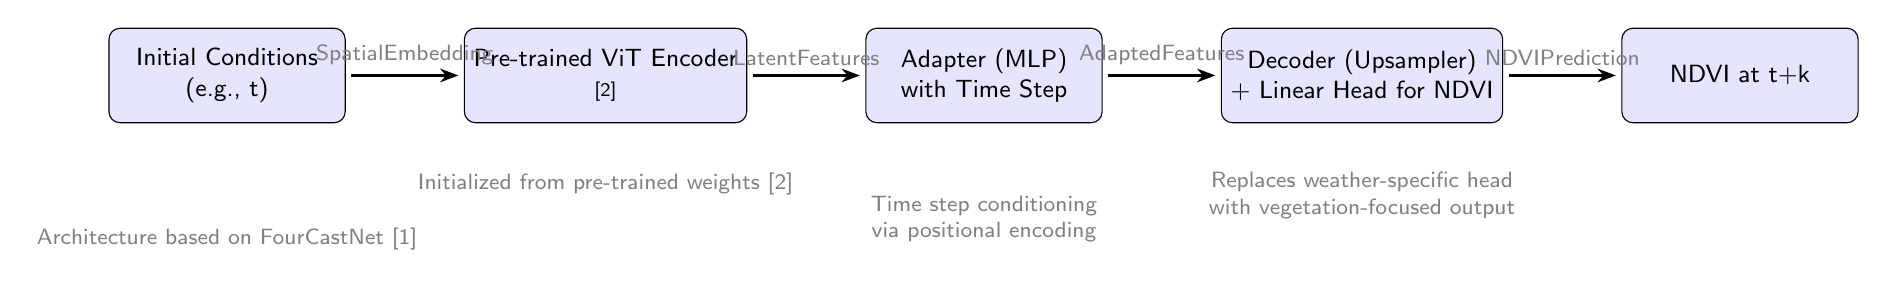
\begin{tikzpicture}[
    node distance=1.5cm,
    block/.style={
        rectangle,
        rounded corners,
        minimum width=3cm,
        minimum height=1.2cm,
        draw=black,
        fill=blue!10,
        font=\sffamily\small,
        align=center
    },
    arrow/.style={
        -Stealth,
        thick,
        shorten >=2pt,
        shorten <=2pt
    },
    label/.style={
        font=\sffamily\footnotesize,
        gray
    }
]

% Nodes
\node (input) [block] {Initial Conditions \\ (e.g., t)};
\node (encoder) [block, right=of input] {Pre-trained ViT Encoder \\ \scriptsize{[2]}};
\node (adapter) [block, right=of encoder] {Adapter (MLP) \\ with Time Step};
\node (decoder) [block, right=of adapter] {Decoder (Upsampler) \\ + Linear Head for NDVI};
\node (output) [block, right=of decoder] {NDVI at t+k};

% Arrows
\draw[arrow] (input) -- node[above, label] {Spatial\\Embedding} (encoder);
\draw[arrow] (encoder) -- node[above, label] {Latent\\Features} (adapter);
\draw[arrow] (adapter) -- node[above, label] {Adapted\\Features} (decoder);
\draw[arrow] (decoder) -- node[above, label] {NDVI\\Prediction} (output);

% Annotations
\node[below=0.5cm of encoder, label] {Initialized from pre-trained weights [2]};
\node[below=0.5cm of decoder, label, align=center] {Replaces weather-specific head \\ with vegetation-focused output};

% Citations
\node[below=1.2cm of input, label, align=center] {Architecture based on FourCastNet [1]};
\node[below=0.8cm of adapter, label, align=center] {Time step conditioning \\ via positional encoding};

\end{tikzpicture}
\end{document}